\documentclass[acmtog]{acmart}
\usepackage{graphicx}
\usepackage{subfigure}
\usepackage{natbib}
\usepackage{listings}
\usepackage{bm}

\definecolor{blve}{rgb}{0.3372549 , 0.61176471, 0.83921569}
\definecolor{gr33n}{rgb}{0.29019608, 0.7372549, 0.64705882}
\makeatletter
\lst@InstallKeywords k{class}{classstyle}\slshape{classstyle}{}ld
\makeatother
\lstset{language=C++,
	basicstyle=\ttfamily,
	keywordstyle=\color{blve}\ttfamily,
	stringstyle=\color{red}\ttfamily,
	commentstyle=\color{magenta}\ttfamily,
	morecomment=[l][\color{magenta}]{\#},
	classstyle = \bfseries\color{gr33n}, 
	tabsize=2
}
\lstset{basicstyle=\ttfamily}

% Title portion
\title{Assignment 5:\\ {}} 

\author{Name:\quad Xiaohan Wu  \\ student number:\ 2019533093
\\email:\quad wuxh@shanghaitech.edu.cn}

% Document starts
\begin{document}
\maketitle

\vspace*{2 ex}

\section{Introduction}
\qquad In HW5, we are required to implement a very basic rigid body simulation involving translation of spheres with collision detection and contact handling between spheres and parallelograms. The program contains 4 basic parts and 1 optional part. The four parts are: 1.Synchronize the simulation and the rendering in OpenGL to show the result in real time.
2.Implement the collision detection between the parallelograms and the sphere.
3.Implement the collision adjustment so that the inter-penetration is within the given tolerance (a small threshold).4.Implement the colliding contact handling between the the parallelogram and the sphere without consideration of rotation.The optional part is: Simulate with multiple spheres simultaneously.
\section{Implementation Details}
\qquad In this section, I will introduce how I implement my program for each part respectively.
\\\indent 1.The realization of moving the scene without considering collisions bases on the concept of momentum.First,we add up with all the force,multipling it with time step dt to get the impulse, then divide it with the mass of the object to get its velocity at that time,also we can get the position of the object.After we finish Sphere::Forward part,for the Sphere::Backward part, it's nearly as same as the previous one except that it is in the inverse order.
\\\indent 2.After making the scene move,we start to detect the collision. To detect the collision between parlgrm and sphere is more difficult than that between sphere and sphere. We have to first calculate the distance between sphere and the parlgrm,comparing it with the radius of the sphere. Then,we have to project the sphere to the parlgrm to judge if the center of the sphere really can be projected onto the parlgrm,or it will also be judeged as failure to collide.To detect the collision between two spheres, we neeed only to calculate the distance between two center positions of the spheres and compare it with the sum of the radius of two spheres.
\\\indent 3.After implementing the previous part,we have to adjust the collision point.As being taught in the class,we first forward the scene with dt.If inter-penetration is detected, then we have to backward and forward the scene back and forth such that time $t_c$ is founded within the tolerance.However, it may occur that whatever we iterate,we can't find such time satisfying the condition. For that situation, we set up a threshold for the time to avoid unbreakable loop.
\begin{figure}[h]
	\centering
	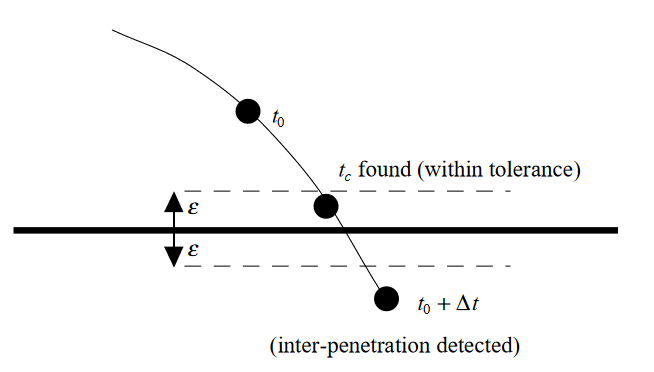
\includegraphics[width=6cm,height=4cm]{adjust.PNG}
\end{figure}
\\\indent 4.After the collision is detected and adjusted, the next step is to handle the collision contact.Before that,we should remember to clear all the transient forces before(this can be easily forgotten.And also pay attention to that we have to clear them after adjusting the collision because the forward and backward still requires the calculation of those forces.)This is the most difficult part in this program.To handle the collision between wall and sphere,we have to first calculate the relative velocity along the surface normal and tangent direction respectily, and multipy them with corresponding epsilon to get the out velocity. Then we can get the delta of the relative velocity to calculate the change of the momentum so that to store that force into the sphere object to be processed in the next time step.Also,we need to pay attention to the supporting force of the surface. What I do in my code is that if the relative velocity of the sphere along the surface normal is samller than the threshold, we calculate the join force of the object and divide it into two directions(along surface normal and tangent). Thus the supporting force is the value of the one along surface normal with opposite direction.(This is an approximate model and not the same as the reality. But for simplicity, we program the code in such a easier way which can also simulate not bad.)
\\\indent To handle the collision between two spheres, I just use the formula mentioned in the class to calculate the impluse between two collided spheres.
\begin{figure}[h]
	\centering
	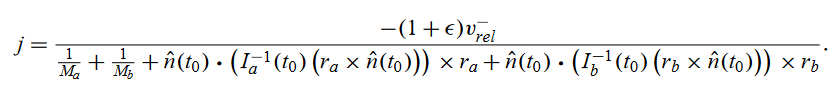
\includegraphics[width=9cm,height=1cm]{formula.PNG}
\end{figure}
\section{Results}
\qquad Below are the results of my programming work.
\begin{figure}[h]
	\centering
	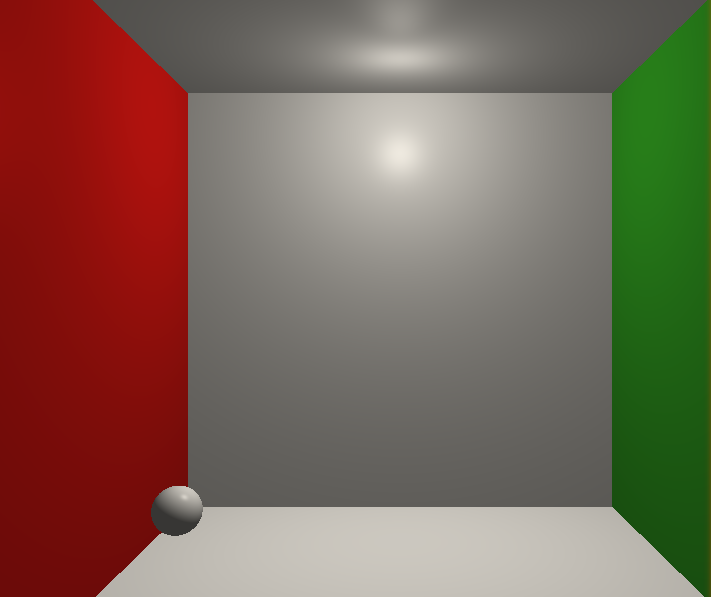
\includegraphics[width=7cm,height=7cm]{output0.png}
\end{figure}
\begin{figure}[h]
	\centering
	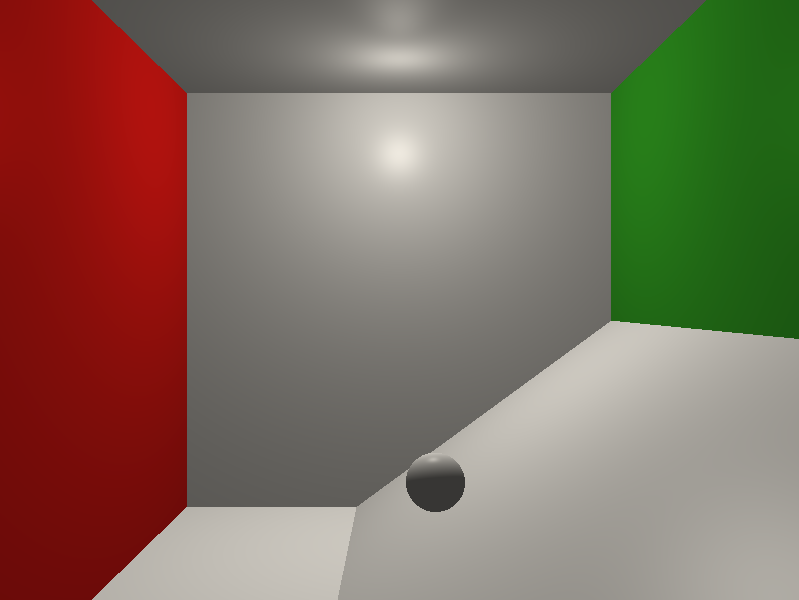
\includegraphics[width=7cm,height=7cm]{output1.png}
\end{figure}
\begin{figure}[h]
	\centering
	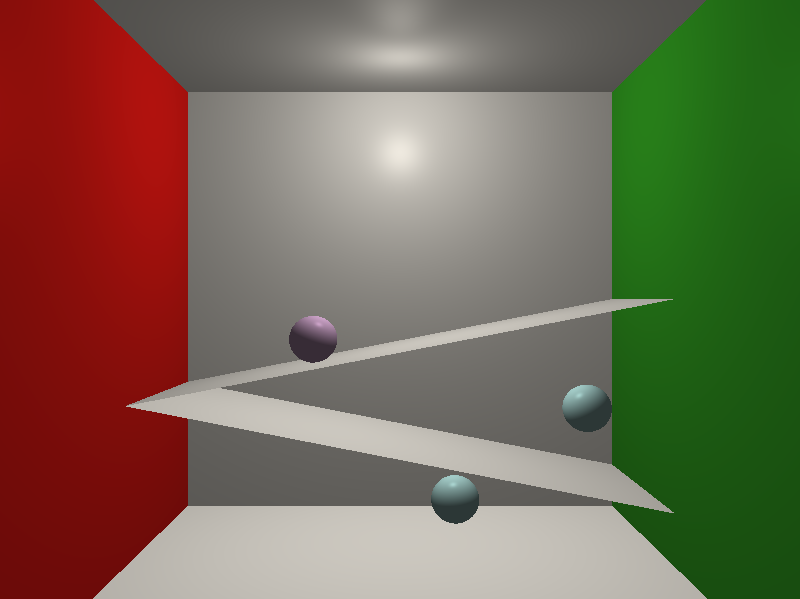
\includegraphics[width=7cm,height=7cm]{output2.png}
\end{figure}
\begin{figure}[h]
	\centering
	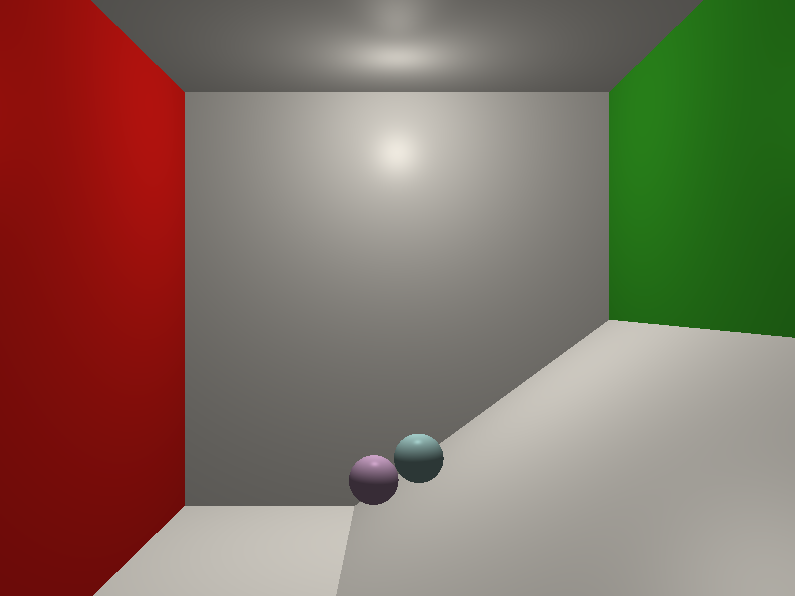
\includegraphics[width=7cm,height=7cm]{output3.png}
\end{figure}
\begin{figure}[h]
	\centering
	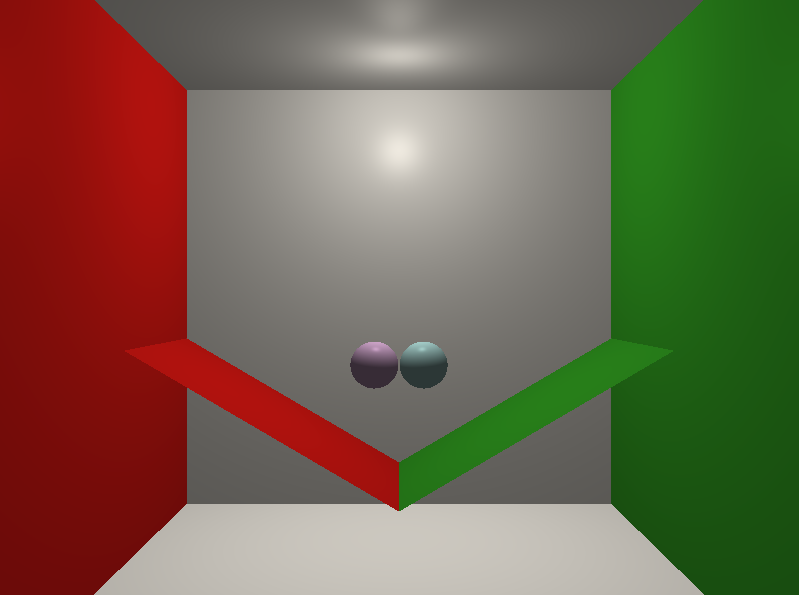
\includegraphics[width=7cm,height=7cm]{output4.png}
\end{figure}


\end{document}
